\section{Lezione 10}%
\label{sub:Lezione 10}
\subsection{Random Walk di Weierstrass nel dettaglio}%
\label{sub:Random Walk di Weierstrass nel dettaglio}
Abbiamo visto che per un camminatore di Weierstrass la forma della distribuzione poteva non essere Gaussiana al variare del parametro $N^2 / b$ (Vedi sezione \ref{sub:Random Walk di Weierstrass}). \\
Rispetto alla lezione 6 adesso si cambia la notazione (Lez6 $\to $ Lez10):
\[
	b\to M \qquad  N \to b
.\]
Quindi adesso $b$ è il parametro dell'ampiezza di salto mentre $M$ è il fattore che smorza il rate. La condizione di rottura del teorema del limite centrale diventa:
\[
    \frac{b^2}{M} > 1
.\] 
Cerchiamo la distribuzione invariante per il camminatore di Weierstrass proprio in questo caso.\\
La probabilità di fare un salto $l$ può essere scritta come:
\[\begin{aligned}
    P(l) = \frac{M-1}{2M}\sum_{J=0}^{\infty} \frac{1}{M^J}\left[\delta (l-b^Ja) + \delta (l+b^Ja) \right]
.\end{aligned}\]
Per capire se è invariante è necessario considerare $n$ salti, farlo nello spazio reale può essere complicato.\\
Ricordiamo le proprietà generali di questo moto random:
\begin{itemize}
    \item Occorrono $\sim M$ salti di $\pm a$ prima di saltare $ba$.
    \item Occorrono $\sim M$ salti di $\pm ba$ ($M^2$ salti lunghi $a$) prima di saltare $b^2a$.
    \item etc \ldots
\end{itemize}
Queste caratteristiche fanno si che il sistema esibisca dei cluster di camminatori attorno alle posizioni dei salti più lunghi (sulla scala temporale di osservazione).
\begin{figure}[H]
    \centering
    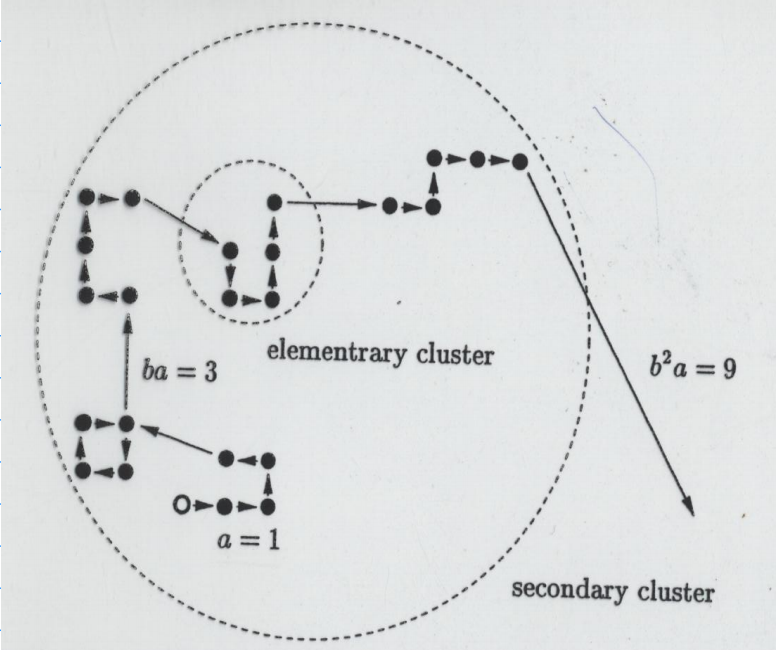
\includegraphics[width=0.4\textwidth]{figures/10_RWWeierstrass.png}
    \caption{\scriptsize Random Walk di Weierstrass ($b=3$, $M=4$): formazione dei Cluster (Paul and Baschangel: Stochastic Process, Springer).}
    \label{fig:figures-10_RWWeierstrass-png}
\end{figure}
\noindent
Proprio per la formazione di questi cluster su scale spaziali diverse il sistema può presentare un comportamento auto-similare.\\
Possiamo notare anche come cambiano i risultati al variare dei parametri $M$ e $b$:
\begin{figure}[H]
    \centering
    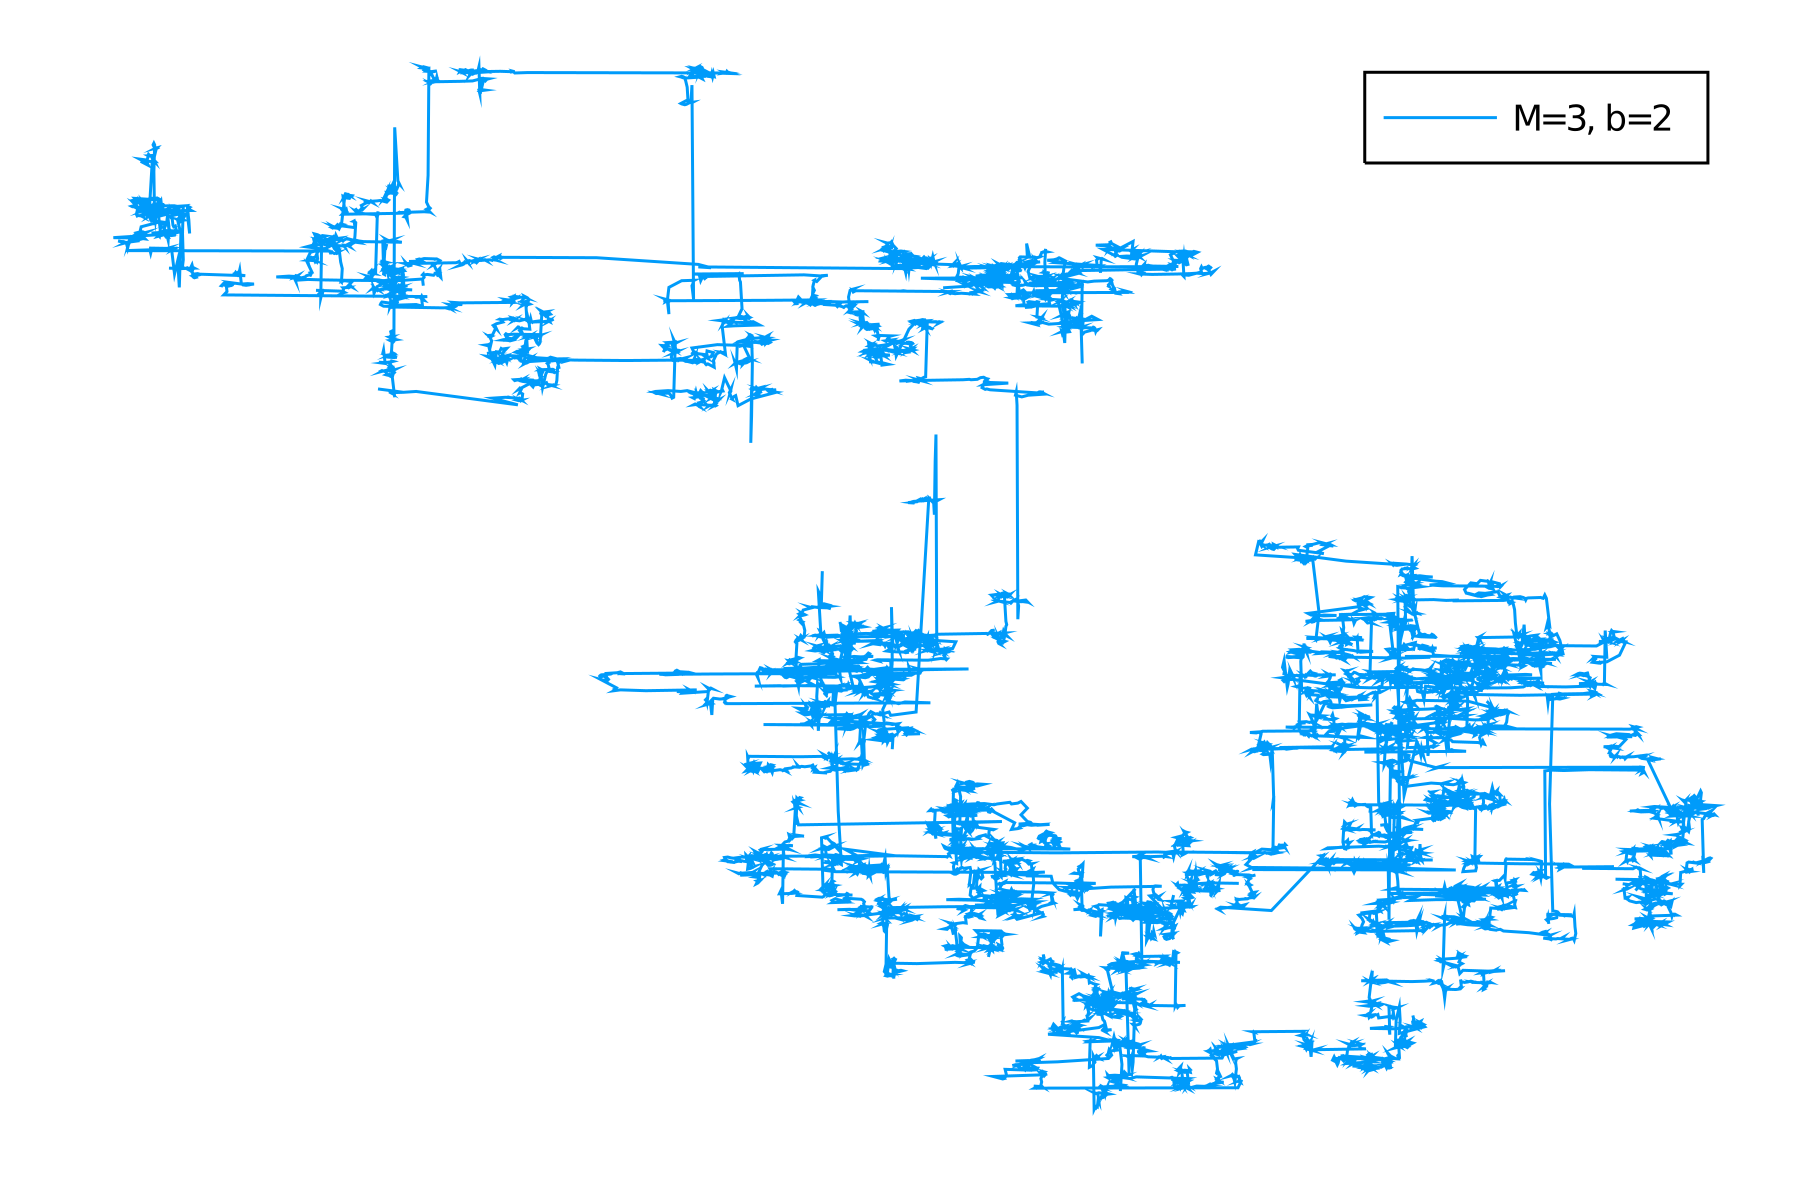
\includegraphics[width=0.45\textwidth]{figures/lez_10_Weier_M_3_b_2.png}
    \caption{\scriptsize Rapporto $b^2 /M = 4 /3 $ (\href{https://github.com/dodogabrie/Sistemi-Complessi/blob/master/python-project/lezione10/Weierstrass_julia.ipynb}{Link al codice}).}
    \label{fig:figures-lez_10_Weier_M_3_b_2-png}
\end{figure}
\begin{figure}[H]
    \centering
    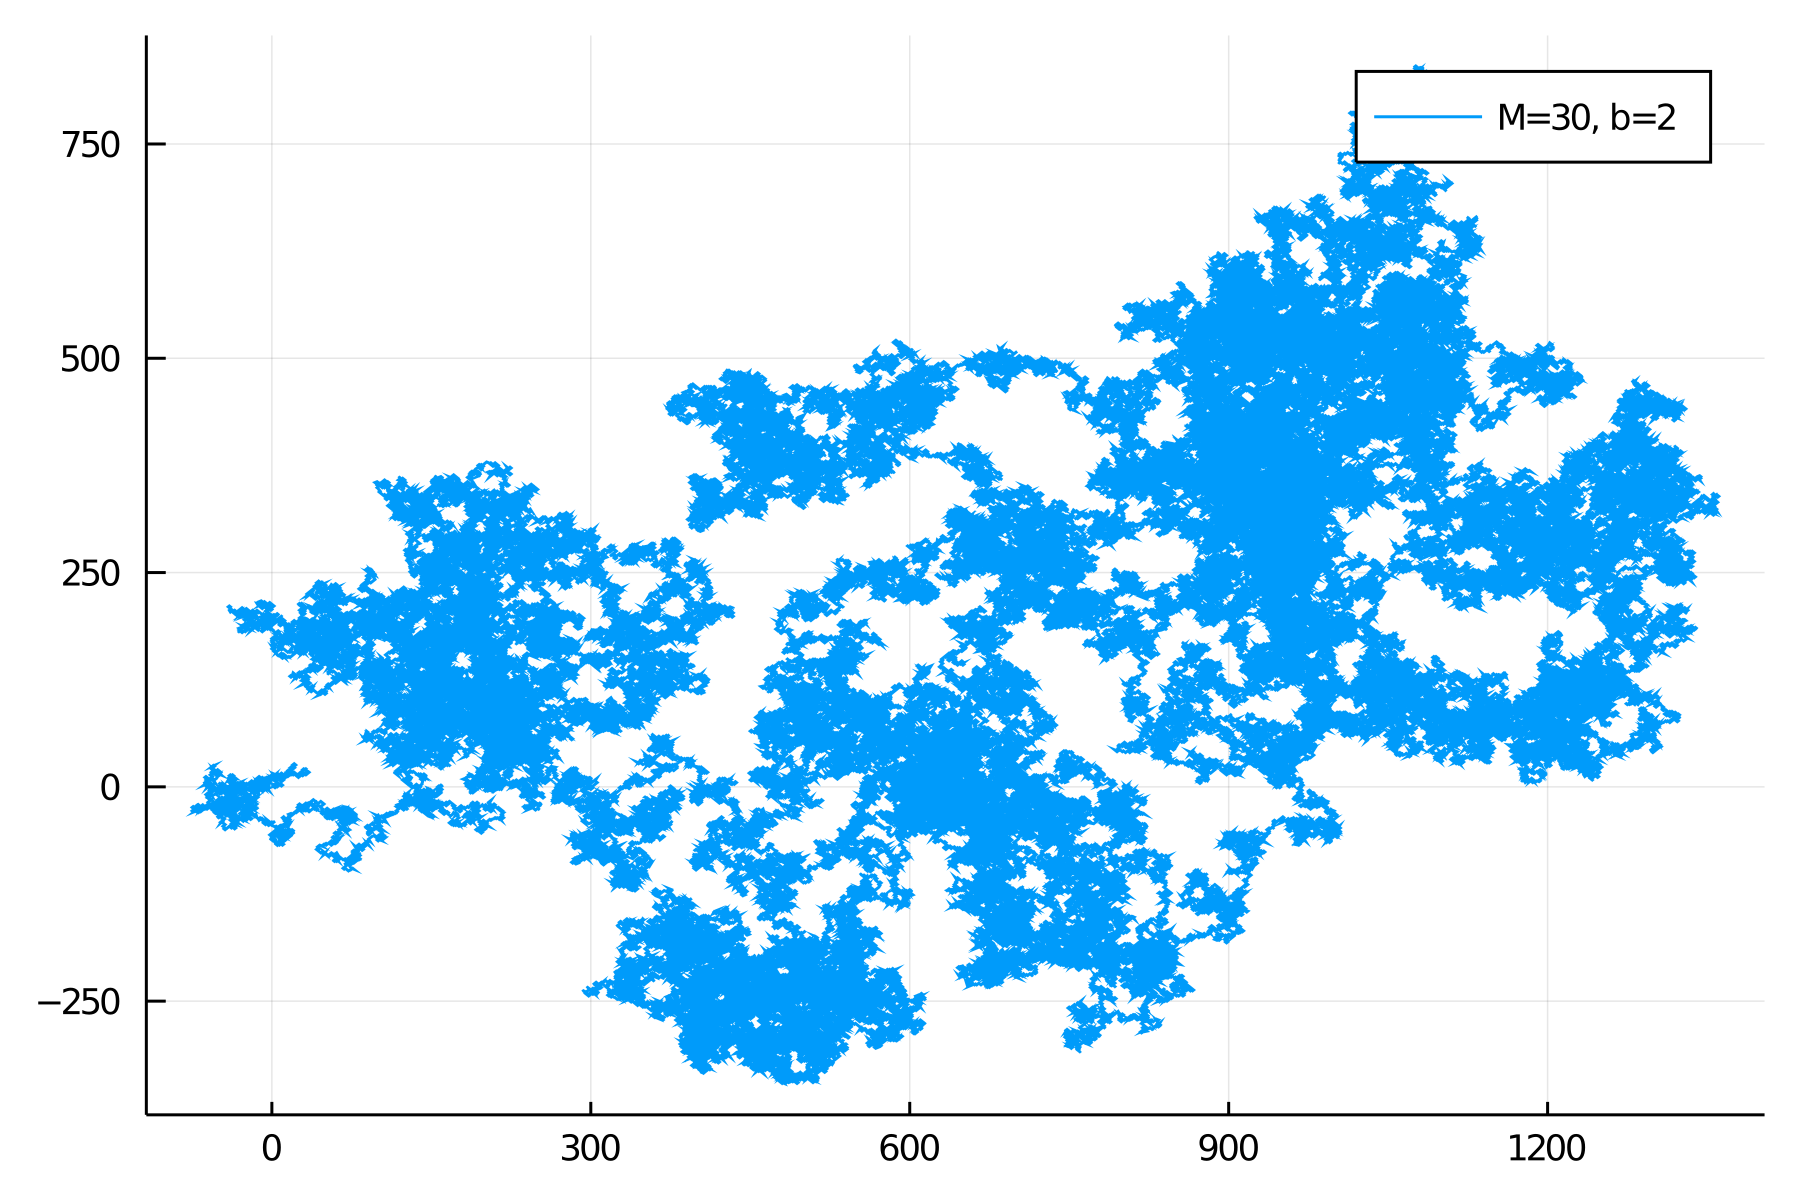
\includegraphics[width=0.45\textwidth]{figures/lez_10_Weier_M_30_b_2.png}
    \caption{\scriptsize Rapporto $b^2 /M = 4 /30$, notiamo come i cluster che si formano siano diversi nei due casi: in questo caso il moto diventa quasi irriconoscibile rispetto ad un RW "normale". (\href{https://github.com/dodogabrie/Sistemi-Complessi/blob/master/python-project/lezione10/Weierstrass_julia.ipynb}{Link al codice}) .}
    \label{fig:figures-lez_10_Weier_M_3_b_2-png}
\end{figure}
\noindent
Mettiamoci nel caso in cui la distribuzione non può essere una Gaussiana e risolviamo per $\left<l^2\right>\to \infty$:
\[
    \left<l^2\right> = \frac{\left(M-1\right)a^2}{M}\sum_{}^{} \left(\frac{b^2}{M}\right)^J\to \infty \quad \text{se }\frac{b^2}{M}>1
.\] 
Per capire se $P(l)$ può essere stabile andiamo in trasformata:
\subsection{Serie di Weierstrass e distribuzione stabile per il RW}%
\label{sub:Serie di Weierstrass e distribuzione stabile per il RW}
Ricordando che:
\[
    P(k) = \left<e^{ikl}\right>
.\] 
Si ottiene:
\begin{redbox}{}
\[
    P(k)  = \int dl P(l) e^{ikl} = \frac{M-1}{M} \sum_{J}^{} \frac{\cos (kb^Ja) }{M^J}
.\]    
\end{redbox}
\noindent
Questa serie è continua ovunque ma non differenziabile rispetto a $k$ se $b>M$.\\
Per dimostrare che $P(l)$ è stabile dobbiamo dimostrare che $P(k)$ è invariante sotto convoluzione. Partiamo osservando come scala $P(k)$ se mandiamo $k\to bk$, questo cambio di scala è interessante perché $b$ è l'unica grandezza fisica che descrive la scala sulla quale avviene il moto del camminatore. 
\[\begin{aligned}
    P(bk) =& \frac{M-1}{M}\sum_{J=0}^{\infty} \frac{1}{M^{J}}\cos (kb^{J+1}a) =\ldots=\\
	   & = M P(k) - \frac{M-1}{M}\cos (ka) 
.\end{aligned}\]
Per arrivare a questa conclusione si è esplicitata la sommatoria di $P(bk)$, moltiplicato e diviso per $M$ e isolato il primo termine della sommatoria.
\begin{redbox}{Equazione per la $P(k)$}
\[
    P(k) = \frac{1}{M}P(bk) + \frac{M-1}{M}\cos (ka) 
.\]     
\end{redbox}
\noindent
Per soddisfare l'invarianza di scala la $P(k)$ deve soddisfare questa equazione. Dividiamo la soluzione in una parte omogenea ed una particolare.
\[
    P(k) = \frac{1}{M}P_0(k) + P_p(k) 
.\] 
Possiamo sviluppare in serie il coseno per trovare la forma della soluzione particolare:
\[
    P_p(k) = \frac{M-1}{M} \sum_{J=1}^{} \frac{(-1)^{J}}{\left(2J\right)!} \frac{(ka)^{2J}}{1-b^{2J} /M} + 1
.\] 
Notiamo subito che la soluzione particolare non è responsabile della divergenza di $\left<l^2\right>$, infatti possiamo calcolare il momento secondo come:
\[
    \left<l^2\right> = - \left.\frac{\text{d} ^2}{\text{d} k^2} P_0(k)\right|_{0}- \left.\frac{\text{d} ^2}{\text{d} k^2} P_p(k)\right|_{0}  
.\] 
La derivata seconda di $P_p$ non diverge:
\[
     \left<l^2\right>_p = \frac{M-1}{M} \frac{a^2}{b^2 /M - 1} < \infty \qquad \text{ con }b^2 /M > 1
.\] 
Quindi è il termine omogeneo di pura scala ad essere responsabile della divergenza.
\begin{greenbox}{Scaling discreto della soluzione omogenea}
\[
    P_0(k) = \frac{1}{M}P_0(bk) 
.\]    
\end{greenbox}
\noindent
Possiamo esprimere la soluzione di questa equazione in funzione di una qualunque $Q(k)$ tale che:
\begin{itemize}
    \item $Q(k) = Q(kb)$ 
    \item $Q(k)$ periodica in $\ln (k)$ con periodo $T = \ln (b)$.
\end{itemize}
Senza riportare i passaggi la soluzione della omogenea è:
\[
    P_0(k) = \left|ka\right|^{\alpha}Q(k) 
.\] 
con:
\[
    \alpha  = \frac{\ln(M)}{\ln(b)} \qquad 0<\alpha <2
.\] 
Che deve essere rispettata per imporre la self-similarità.\\
Valutando i termini della soluzione, $P_p$ e $P_0$, quando $k\to 0$ si nota che sopravvivono solo:
\begin{itemize}
    \item Il termine unitario nella $P_p$ (il termine più rilevante nella sommatoria va a zero come $k^2$).
    \item L'intera soluzione omogenea ($\alpha < 2$)
\end{itemize}
Per $k\to 0$ si ha quindi che:
\[
    P(k) \sim 1 - c(\alpha) \left|ka\right|^\alpha
.\] 
Per ricondurci ad una forma del tipo Levy dobbiamo trovare il modo di esprimere il $\log P(k) $, approssimiamo allora la $P(k)$ ottenuta per $k\to 0$ come esponenziale (visto che corrisponde ai primi due termini dello sviluppo di quest'ultimo).
\[
    P(k) \sim \exp\left(-c(\alpha) \left|k a\right|^\alpha\right)
.\] 
Quindi:
\[
    \ln (P(k) ) = -c(\alpha) \left|k a\right|^\alpha
.\] 
Che è effettivamente una distribuzione di Levy con $\alpha  = \ln M /\ln b$. Quindi la distribuzione $P(l)$ è stabile per tutti i valori di $b^2 /M$.
\clearpage
